% !TeX root = ../../thesis.tex
\chapter{Nucleation probability assessment - a phase field methodology}\label{ch_NPA_PF_methodology}

\section{Introduction}
This chapter develops a methodology to obtain insight about the nucleation barrier from the equilibrium stable shapes of particles on a planar support in 2D. The developed multi-phase phase field model is used to obtain the interface-energy-minimizing shapes and the below described \textit{domain scaling} is then used to find the shape factor. As recalled in the next section, the shape factor $S$ is closely related to the nucleation barrier of the heterogeneous nucleus (having the equilibrium shape), thus to the nucleation probability. 

Even though this method was primarily developed to bring insight into the anisotropy in the nucleation barrier as a function of the orientations of both the substrate and nucleus (which is in principle possible), later it was decided to rather use the Winterbottom construction for this purpose (in Chapter~\ref{ch_paper2}), because it was much more efficient. Regardless, the method presented in this chapter retains its usefulness because it can be used without any assumption on the shape itself (except for the contact angles it has with the substrate). This was exploited in solving a problem of heterogeneous nucleation on top of a grain boundary intersecting surface of a polycrystalline substrate. 

Grain boundaries in nanocrystalline catalytic materials can be seen as a source of surface chemical functionality~\cite{Landau2014}. They are defects in the crystalline structure, hence they are associated with certain excess energy, which makes them active sites for many chemical or electrochemical processes~\cite{Landau2014,Xu2024,Wang2024}, including nucleation. 

In order to find the equilibrium stable shape for arbitrary orientation and wetting conditions using the Moelans' multi-phase field model~\cite{Moelans2008} described also in chapter~\ref{ch_paper1}, it was necessary to implement two model extensions: volume conservation and such boundary conditions, which allow control of the interface inclination at the domain boundary. That way, the shape could be simulated in a two-phase 2D system as long as the contact angles were known.

%The used model represents wetting of a plane by a crystal and extends the Moelans' multi-phase field model described in chapter~\ref{ch_paper1} by the following: volume conservation using the fictitious concentration field approach and the general Neumann boundary conditions to control the interface inclination at the domain boundary. 

The combination of methods used to obtain the shape factors (phase field and domain scaling) utilizes that the interface in phase field method is implicitly tracked, i.e. it evolves without any assumption on its position. Additionally, it makes use of the fact, that in the simulated geometry, the total energy of the system is in fact the total particle-liquid interface energy. Advantage of the method is that it does not a-priori assume any shape, it is thus in principle usable for non-analytic cases, where the solution is not known, e.g. a particle on a grain boundary.

The below sections first recall some fundamentals relevant for the subsequently described \textit{domain scaling} methodology. Then follows technical description of how the phase field model was extended to conserve volume and to have control over the inclination of interfaces at the domain boundary. Then, some details about the numerical implementation are included, followed by validations of the implementation in terms of how well the contact angles are reproduced for straight interface and the domain scaling methodology is then validated for circular segments with different contact angles, which is the case of heterogeneous nucleation with isotropic interface energy in 2D. The domain scaling method is then applied to the case with a particle with isotropic interface energy on top of a grain boundary intersecting a substrate surface. Limitations and prospects of this approach are assessed based on the results.


%The below procedure assumes a 2D particle sitting on top of a line, the contact angles on the left and right are known. It is assumed that the environment surrounding the particle is liquid and the particle-liquid energy is anisotropic. The contact angles are determined using the Young's equation. 
%
%The following sections describe how the phase field result can be used to bring insight about the nucleation barrier using scaling of simulation domain, which is a kind of post-processing of the results. 


\section{Fundamentals}
In 2D, the Gibbs free energy difference upon a nucleus insertion in the system is due to competition between area and line energy contributions (see also Figure \ref{fig_DG_2D_sketch}). Be $A_{hom}$ the nucleus area and its interface be described by a parametric curve $\mathcal{C}$. In the isotropic case, $\mathcal{C}$ is a circle and the interfacial contribution is simply $\sigma L$, where $L=2\pi R$ is the interface length and $\sigma$ the isotropic specific interface energy. The Gibbs free energy difference of a free nucleus is then (with $\Delta G_A$ being the 2D equivalent of bulk driving force, i.e. with units \unit{J/m^2})
\begin{align}
	\Delta G_{hom} &= -\Delta G_A A_{hom} + \sigma L \\
	\label{eq_DG_hom_iso}	&= (-\Delta G_A R^2 + 2R\sigma)\pi \,,
\end{align}
which implies the critical radius
\begin{equation} \label{eq_crit_radius_2D}
	R_c = \frac{\sigma}{\Delta G_A}
\end{equation}
and critical nucleation barrier
\begin{equation} \label{eq_nucl_barr_hom_2D}
	(\Delta G_c^*)_{hom} = \hat{A}_{hom}\frac{\sigma^2}{\Delta G_A}\,,
\end{equation}
where the non-dimensional nucleus area is $\hat{A}_{hom}=A_{hom}/R^2=\pi$.

\begin{figure}
	\centering
	\includegraphics[width=0.5\textwidth]{DG_vs_radius_2D.pdf}
	\caption[Dependence of the total energy change on the radius of the inserted nucleus in 2D]{Schematic dependence of the total energy change on the radius of the inserted nucleus in 2D.}
	\label{fig_DG_2D_sketch}
\end{figure}

In the heterogeneous nucleation, the shape factor $S(\theta)=A_{het}/A_{hom}$ scales the homogeneous total energy change upon nucleus insertion $\Delta G_{hom}$ as
\begin{equation}\label{eq_DG_het_2D}
	\Delta G_{het} = S(\theta)\Delta G_{hom} \,,
\end{equation}
which for the heterogeneous nucleation barrier implies
\begin{equation}\label{eq_nucl_barr_het_2D}
	(\Delta G_c^*)_{het} = S(\theta)(\Delta G_c^*)_{hom}\,.
\end{equation}
The nucleus radius is equal in both homogeneous and heterogeneous nucleation.

%When the interface energy is inclination-dependent $\sigma(\theta)=\sigma_0 f(\theta)$, the interface energy contribution is a line integral $\int_\mathcal{C} \sigma(\theta) \mathrm{d}l$, which can be expressed in analogy with the 3D case~[Mariaux2010] as ($X_0$ being the generalized radius of the Wulff shape with area $A_{hom}^{ani}$)
%\begin{equation}
%	\int_\mathcal{C} \sigma(\theta) \mathrm{d}l = \frac{2\sigma_0}{X_0}A_{hom}^{ani} \,,    
%\end{equation}
%which eventually allows to write the Gibbs free energy difference of a free nucleus
%\begin{equation}\label{eq_DG_hom_aniso}
%	\Delta G_{hom}^{ani} = (-\Delta G_A X_0^2 + 2\sigma_0 X_0)\hat{A}_{hom}^{ani} 
%\end{equation}
%and further its nucleation barrier
%\begin{equation} 
%	(\Delta G_c^*)_{hom} = \hat{A}_{hom}^{ani}\frac{2\sigma^2}{\Delta G_A}\,.
%\end{equation}
%In the heterogeneous anisotropic nucleation the difference in Gibbs free energy is like in equation~\eqref{eq_DG_het_2D}, having $\Delta G_{hom}^{ani}$ as in~\eqref{eq_DG_hom_aniso} and the nucleation barrier like in~\eqref{eq_nucl_barr_het_2D}, only with modified shape factor $S$ correspondingly to the Wulff shape.
%\begin{equation} \label{eq_DGcrit_het_aniso}
%	(\Delta G_c^*)_{het} = S\hat{A}_{hom}^{ani}\frac{2\sigma^2}{\Delta G_A}\,.
%\end{equation}
%For nucleation with both isotropic and anisotropic energy, the dependence of the total energy change on the particle radius has the same form~\eqref{eq_DG_hom_iso} and~\eqref{eq_DG_hom_aniso}, which is sketched in Figure~\ref{fig_DG_2D_sketch}.


\section{Methodology}
%\subsection{Principle}
%The critical nucleation barrier is the maximal possible energy change attributed to insertion a nucleus of a particular shape, interface energy and in the present supersaturation (bulk driving force in general). 
The simulated system geometry is sketched in Figure~\ref{fig_sketch_domain_scaling_PF}. A two-phase system of a particle in a liquid was described by two phase field variables in Moelans' model, one representing the liquid parent phase ($\eta_1$) and the second ($\eta_2$) representing the particle (possibly with anisotropic interface energy). The bottom domain boundary then represents the substrate and the interface inclination $\vartheta_L,\vartheta_R$ in the two contact points is controlled by the boundary condition as indicated in the figure.
\begin{figure}
	\centering
	\includegraphics[width=0.8\textwidth]{sketch_geometry_PF_NPA.pdf}
	\caption[Sketch - PF simulation domain geometry to obtain equilibrium stable shape of a particle on a plane]{Sketch of the geometry in the phase-filed simulations used in the domain scaling methodology for shape factor assessment. The symbols $\vartheta_L,\vartheta_R$ denote tangent angles in the contact points and $\theta_L,\theta_R$ the normal ones. The two intervals on the bottom domain boundary with the different interface inclination imposed are indicated  by blue color on the left half of the domain and by magenta on the right one (note that $\eta_1$ has analogous boundary conditions which must be consistent). $l_{GB}$ is the length of the grain boundary interval between the contact points. $\sigma_P$ is the particle-liquid interface energy.}
	\label{fig_sketch_domain_scaling_PF}
\end{figure}

Volume conservation was assured using the fictitious concentration field described in the section~\ref{sec_volume_cons_PF_ch_NPA_PF}. 

The particle-liquid interface energy $\sigma_P$ was assumed, together with the contact angles $\vartheta_L, \vartheta_R$ between the solid-liquid interface and the bottom domain boundary. How these angles were imposed is described in section~\ref{sec_general_NBC_ch_NPA_PF}.

The domain scaling methodology is in fact a post-processing of the result of phase field simulation. By the result, it is meant the phase fields corresponding to the liquid and to the particle within the simulation grid. Then, the grid spacing $\Delta x$ is scaled and the model parameters are re-computed accordingly. The particle area fraction $\xi=A_P/A_D$ in the scaled system remains the same, but its area $A_P$ and perimeter are scaled accordingly. Using the (unchanged) phase fields and re-computed parameters, the total interface energy is re-evaluated by the free energy functional $F(\eta,\nabla\eta)$ for the new scale. The domain scaling is sketched in Figure~\ref{fig_domain_scaling}a. 

\begin{figure}
	\centering
	\includegraphics[width=\textwidth]{combined_sketch_domain_scaling.pdf}
	\caption[Nucleation barrier determination using domain scaling]{Nucleation barrier determination using domain scaling. In (a) sketch of domain scaling. The area fraction of the particle is preserved, as well as the number of grid points $N_x, N_y$. $A_i$ are scaled areas of the domain and $\Delta x_i$ is the i-th scaled grid spacing in meters. In (b) the energy contributions were plotted for each $\Delta x_i$, the barrier being denoted by black crosses and the critical nucleation barrier determined by fitting of parabolic function is indicated by red diamond.}
	\label{fig_domain_scaling}
\end{figure}	

Note that the free energy functional $F(\eta,\nabla\eta)$ only accounts for the solid-liquid interface energy, but in the total energy change upon nucleus insertion, there must be included also the term representing the replacement of the former planar substrate-liquid interface with specific energy $\sigma_S$ by the grain boundary: $l_{GB}(\sigma_{GB}-\sigma_S)$. Because the Young's equation for triple junctions of isotropic interfaces reads
\begin{equation}\label{eq_young_iso}
	\sigma_S = \sigma_{GB}+\sigma_P\cos(\vartheta) \,,
\end{equation}
the grain-boundary-energy term can thus be written as $l_{GB}(\sigma_{GB}-\sigma_S)=-l_{GB}\sigma_P\cos(\vartheta)$, which allows us to disregard the values of the substrate and grain boundary energy. In the phase field simulation, the distance between the contact points is interpreted as $l_{GB}$ (see Figure~\ref{fig_sketch_domain_scaling_PF}) and the above term is added to the total interface energy change upon the nucleus insertion $\Delta G_\sigma$, hence when denoting the free energy functional as $F(\eta,\nabla\eta)$ it can be written
\begin{equation}
	\Delta G_\sigma = F(\eta,\nabla\eta) - l_{GB}\sigma_P\cos(\vartheta) \,.
\end{equation}
Note that $l_{GB}$ is necessarily scaled as well during the domain scaling procedure.

The above procedure provided the total interface energy change upon the particle insertion as function of the length scale ($\Delta x_i$ in Figure~\ref{fig_domain_scaling}a). Even though it is not the particle radius as in~\eqref{eq_DG_hom_iso}, the grid spacing has the same physical dimension (length), which assures that the order of the polynomial $\Delta G(\Delta x) = a(\Delta x) - b(\Delta x)^2$ is the same as in~\eqref{eq_DG_hom_iso}.

When the driving force $\Delta G_A$ is explicitly assumed, the bulk energy contribution $\Delta G_B$ to the energy change can be computed using each of the absolute values of the scaled particle area $A_P(\Delta x_i)$ as $\Delta G_B(\Delta x_i)=\Delta G_A A_P(\Delta x_i)$. Because the interface energy contribution $\Delta G_\sigma(\Delta x_i)$ was already computed for each scaled system, it is possible to subtract the two to obtain the total energy change in insertion of those particles, as is shown in Figure~\ref{fig_domain_scaling}b and below
\begin{equation}
	\Delta G(\Delta x_i) = \Delta G_B(\Delta x_i) - \Delta G_\sigma(\Delta x_i)
\end{equation}
 In Figure~\ref{fig_domain_scaling}b, there were multiple scaling steps taken for illustration, but with the simple parabolic dependence of $\Delta G(\Delta x_i)$ in 2D, only 3 points would suffice to unambiguously determine its parameters. Finding the critical nucleation barrier $\Delta G^*_c$, i.e. value of the parabola maximum is then trivial. 

The critical nucleation barrier of the investigated heterogeneous equilibrium shape was thus found. However, a more practical quantity is the corresponding shape factor $S$, which can then be obtained from equations~\eqref{eq_nucl_barr_hom_2D} and~\eqref{eq_nucl_barr_het_2D} as
\begin{equation} \label{eq_NPA_PF_formula}
	S = (\Delta G_c^*)\frac{\Delta G_A}{\hat{A}_{hom}\sigma_0^2} \,.
\end{equation}
Note, that one needs to know the non-dimensional area of the isolated equilibrium shape $\hat{A}_{hom}=A_{hom}/R^2$. Essentially, that is an area of the isolated Wulff shape of unit radius (in this study it was obtained numerically from Wulff shapes plotted with fine resolution).

Recall, that the contact angles of the particle with the substrate were the input to the phase field simulation, hence the obtained shape factor $S$ is a function of the particular assumed conditions. 

The domain scaling procedure does not depend on whether the interface energy was isotropic or anisotropic, because the used formulas leading to~\eqref{eq_NPA_PF_formula} are equal in the two cases~\cite{Mariaux2011}. Only in the case with inclination-dependent interface energy more steps are required in evaluation of the free energy functional $F(\eta,\nabla\eta)$ because the formulas for model parameters are more complicated than in the isotropic case.

\section{Model}
Because the Moelans' model with anisotropic interfaces was already extensively introduced in section~\ref{sec_Models}, this section covers only the necessary extensions to simulate the system as sketched in Figure~\ref{fig_sketch_domain_scaling_PF}, 

	\subsection{General Neumann boundary conditions to control interface inclination at domain boundary}\label{sec_general_NBC_ch_NPA_PF}
	This model extension was inspired by~\cite{Granasy2007}. It allows to control the interface inclination angle $\phi$ at the boundary, which thus becomes an input parameter. The principle is explained using a single phase field $\eta(\bm{r})$. 
	First, we remark that the standard Neumann boundary conditions $\nabla\eta\cdot\bm{n_D}=0$ must be a special case of the general Neumann boundary conditions ($\bm{n_D}$ is the domain boundary normal). The regular Neumann boundary condition implies perpendicularity of the phase field gradient to the domain boundary normal. In other words, the interface is perpendicular to the domain boundary. Generally, we can write $\bm{n_D}\cdot \nabla\eta=|\nabla\eta|\cos(\phi)$. In the model by Granasy~\cite{Granasy2007}, the local magnitude of phase field gradient may be expressed using the local phase field value, giving rise to the following expression for the boundary condition
	\begin{equation}
		\bm{n_D}\cdot \nabla\eta=\frac{\cos(\phi)}{\delta\sqrt{2}}\eta(1-\eta)\,,
	\end{equation}
	where $\delta$ is the interface width. At the domain boundary, the gradient $\nabla\eta$ is expressed as a polynomial, which allows straightforward implementation of the condition, especially in rectangular simulation domains.
	
	In Moelan's model, the interface normal between the phase fields $\eta_i,\,\eta_j$ denoted $\bm{n}_{i,j}$ is defined as local difference in neighboring phase field gradients (see equation~\ref{eq_def_inclination}). In the spirit of the introductory example we can write
	\begin{equation}
		\bm{n_D}\cdot\bm{n}_{i,j} = \cos(\phi) \quad \implies \quad \bm{n}\cdot(\nabla\eta_i-\nabla\eta_j) = |\nabla\eta_i-\nabla\eta_j|\cos(\phi) \,.
	\end{equation}
	Now we have single boundary condition with the correct physical interpretation (fixed inclination angle at the boundary) but because the governing equations are solved for the phase fields, a set of equivalent boundary conditions (one for each phase field) must be derivable from the above. In these independent boundary conditions, it must be possible to express the gradient magnitude (the introductory example finds a polynomial of local phase field values equal to the gradient magnitude). \\
	The first problem (i.e. coupling in the boundary conditions) would be solved if one gradient could be written as a function of the other and vice versa. However, this dependence is non-analytical for all $\gamma_{i,j}\neq1.5$. For $\gamma_{i,j}=1.5$ it is simply $\eta_i = 1-\eta_j$ and therefore also $\nabla\eta_i=-\nabla\eta_j$.~\cite{Moelans2008} \\
	The second problem (i.e. the expression for gradient magnitude) is also enabled by the choice $\gamma=1.5$, as in such a case there have been in 1D derived the analytic expressions for the gradients in $\nabla\eta_i,\nabla\eta_j$ as functions of the phase field values~\cite{Moelans2008}, similar to those in~\cite{Granasy2007}. To generalize them into higher dimensions, several steps need to be made: 
%	1D system with 2 phase fields holds
%	
%	Validity of the last equation sign in 2D and 3D (in systems with 2 phase fields) can be checked using the expressions in~\cite{Moelans2008} as follows: 
	the equation 7 from~\cite{Moelans2008} for 2D/3D writes
	\begin{equation}
		mf_0(\eta_i, \eta_j) + \frac{\kappa_{i,j}}{2} \left[ |\nabla \eta_i|^2 + |\nabla \eta_j|^2 \right] = 0 \,.
	\end{equation}
	From this, the 2D/3D equivalents of equations 8a and 8b can be written, where $\frac{\mathrm{d}\eta}{\mathrm{d}x}$ is replaced by $|\nabla\eta|$
	\begin{equation}\label{eq_PFgradient_analytic_2}
		\begin{split}
			|\nabla\eta_{i}| &= \sqrt{\frac{2mf_0}{\kappa_{i,j}\left[1 + \left( \frac{\mathrm{d} \eta_j}{\mathrm{d} \eta_i} \right)^2\right]}} \\
			|\nabla\eta_{j}| &= \sqrt{\frac{2mf_0}{\kappa_{i,j}\left[1 + \left( \frac{\mathrm{d} \eta_i}{\mathrm{d} \eta_j} \right)^2\right]}} \,.
		\end{split}
	\end{equation}
	Assuming $\gamma_{i,j}=1.5$ implies $\eta_i = 1-\eta_j$, hence $\left( \frac{\mathrm{d} \eta_j}{\mathrm{d} \eta_i} \right)^2=1$. In addition to that, the homogeneous free energy density $f_0(\eta_{i},\eta_{j})$ can be expressed as a function of only one of the two fields (see the equation 19 from~\cite{Moelans2008})
	\begin{equation}
		f_0(\eta_{i},1-\eta_{i}) = 2\eta_{i}^2(1-\eta_{i})^2 \,.
	\end{equation}
	After substitution in~\ref{eq_PFgradient_analytic_2}, the gradients are expressed in 2D/3D as functions of the respective field values
	\begin{equation} \label{eq_PFgradient_analytic}
		\begin{split}
				|\nabla\eta_i| &= \sqrt{\frac{2m}{\kappa_{i,j}}}\eta_i(1-\eta_i)  \\
				|\nabla\eta_j| &= \sqrt{\frac{2m}{\kappa_{i,j}}}\eta_j(1-\eta_j)  \,.
			\end{split}
	\end{equation}
	
	In systems with more than two phase fields, the general expression for the gradient magnitude is more complex. However, the same relations are satisfied far enough from the triple junction. \\
	With the above, we can thus write
	\begin{equation}
		\begin{split}
			\bm{n}\cdot(\nabla\eta_i-\nabla\eta_j) &= 2\bm{n}\cdot\nabla\eta_i = 2|\nabla\eta_i|\cos(\phi) \\ &= -2\bm{n}\cdot\nabla\eta_j = -2|\nabla\eta_j|\cos(\phi) \,,
		\end{split}
	\end{equation}
	which provides very similar BC like in the introductory example for each of the two phase fields.\\
	The only way how to use these relations is to have $\gamma_{i,j}=1.5$. In the case of inclination-dependent interface energy $\sigma_{i,j}(\theta_{i,j})=\sigma_{i,j}^0h_{i,j}^\sigma(\theta_{i,j})$, it is necessary to express the anisotropy fully by the parameter $\kappa_{i,j}(\theta_{i,j})$, i.e. to use the IWvK model.
	
	\subsection{Volume conserving multi phase field models}\label{sec_volume_cons_PF_ch_NPA_PF}
	There are several approaches which accomplish the volume conservation of some species or phases. Each has its drawbacks though. It was not clear which of the possible approaches was the most convenient for coupling with inclination-dependent interface energy in curvature-driven systems.
	
	Three conceptually different solutions can be used in a multi-phase field model, which are known to the author: Cahn-Hilliard equation, Lagrange multipliers and fictitious concentrations field. 
	
	In order to bring insight into the impact of interface energy anisotropy in textures formation, a parameter study would be needed involving many simulations. Moreover, the intended application with anisotropic interface energy involves complicated driving force terms, hence a less computationally demanding option than the Cahn-Hilliard equation was seeked, because that one is a partial differential equation of 4-th order in space. 
	
	The approach using Lagrange multipliers to conserve volume was thoroughly considered, but eventually it was found out that for Moelan's model it is not a suitable solution. The reason is that the volume of a single phase/grain is defined using all other phase fields, which introduces excessive computational complexity in application of the principles leading to volume conservation. All related details and explanations can be found in Appendix~\ref{ch_lagrange_multipliers_PF}.
	
	The approach using a fictitious concentration field was eventually assessed as the most convenient one. It is not new in combination with Moelans' multi-phase field model (see e.g.~\cite{Yadav2016,Yadav2018vol_cons}). It is briefly reviewed in the following subsection. 
		
		\subsubsection{Fictitious concentration field}
		The idea in the fictitious concentration field approach to conserve volume of a phase field is to couple the Allen-Cahn equation to a conserved concentration field in such a way, that the change in phase fraction is only possible with exchange of species between phases. If the concentration of the independent species is set to equilibrium value and the energy valley is steep enough, no phase transformation occurs and the volume of the phase fraction should be conserved through the system. 
		
		In the description below, it is assumed that there are two phases, one solid and the other liquid.
		
		The free energy functional is then
		\begin{equation}
			F_{cons} = \int_V \left[ f_{hom}(\vec{\eta},\nabla\vec{\eta},c) + f_{grad}(\vec{\eta},\nabla\vec{\eta}) \right] \mathrm{d}V \,,
		\end{equation}
		with   
		\begin{align}
			f_{hom}(\vec{\eta},\nabla\vec{\eta},c)  &= f_0(\vec{\eta},\nabla\vec{\eta}) + f_{chem}(\vec{\eta},c) \\
			f_{chem}(\vec{\eta},c) &= h_S(\vec{\eta})f_S(c) + h_L(\vec{\eta})f_L(c)
		\end{align}
		$h_S(\vec{\eta}), h_L(\vec{\eta})$ are solid and liquid interpolation functions. Assuming that the solid phase is composed of $s$ phase fields $\eta_{S1},\eta_{S2},\dots,\eta_{Ss}$ and the liquid phase of $l$ phase fields $\eta_{L1},\eta_{L2},\dots,\eta_{Ll}$ we can write
		\begin{align}
			h_S(\vec{\eta}) &= \frac{\sum_i^s \eta_{Si}^2}{\sum_i^s \eta_{Si}^2 + \sum_j^l \eta_{Lj}^2}   \\
			h_L(\vec{\eta}) &= \frac{\sum_j^l \eta_{Lj}^2}{\sum_i^s \eta_{Si}^2 + \sum_j^l \eta_{Lj}^2} \quad .
		\end{align}
		Parabolic energy approximation will be used for the concentration dependence of the homogeneous phase free energy densities $f_S(c), f_L(c)$ as
		\begin{align}
			f_S(c_S) &= A(c_S-c_{S,eq})^2 \\
			f_L(c_L) &= B(c_L-c_{L,eq})^2 \,.
		\end{align}
		An ideal solution approximation was adopted.
		
		The governing equations for two phase fields are then
		\begin{align} \label{eq_governing_eq_volcons_1}
			\frac{\partial \eta_1}{\partial t} &= -L\left[\frac{\partial f_0}{\partial \eta_1} - \nabla\cdot \frac{\partial F}{\partial (\nabla\eta_1)} + \frac{\partial h_S}{\partial \eta_1}[f_S(c_S) - f_L(c_L) - (c_S-c_L)\mu] \right] \\
			\frac{\partial \eta_2}{\partial t} &= -L\left[\frac{\partial f_0}{\partial \eta_2} - \nabla\cdot \frac{\partial F}{\partial (\nabla\eta_2)} + \frac{\partial h_S}{\partial \eta_2}[f_S(c_S) - f_L(c_L) - (c_S-c_L)\mu] \right] \\
			\mu &= 2A(c_L-c_{L,eq})\\
			\frac{\partial c}{\partial t} &= \frac{D}{A}\Delta\mu  = 2D\Delta(c_L-c_{L,eq})  \label{eq_governing_eq_volcons_end}
		\end{align}
		where the diffusion coefficient $D$ is a constant.
		
		The interpolation functions have the following property
		\begin{equation}
			\frac{\partial h_S}{\partial \eta_p} = -\frac{\partial h_L}{\partial \eta_p}
		\end{equation}
		
		%The difference in grand potential in the solid and liquid phase is the driving force for change of the phase fraction. It is assumed that $A=B$ and thus
		%\begin{equation}
		%	f_S(c_S) - f_L(c_L) - (c_S-c_L)\mu = 
		%\end{equation}

\section{Numerical implementation}
The numerical approach to solving the governing equations~\ref{eq_governing_eq_volcons_1}-\ref{eq_governing_eq_volcons_end} was the same as in the Chapter~\ref{ch_paper1}, i.e. finite difference method of the second and of first order for the spatial and temporal derivatives, respectively. Own solver was written in MATLAB.

The Appendix~\ref{ch_numerical_implementation} contains the necessary modifications to the finite-difference algorithm when implementing the general Neumann boundary conditions. Eventually, the changes affected all the finite difference operators (standing in place of unidirectional or mixed derivatives and laplacian), but only in the parts of the matrices, which involve the nodes at the domain boundary.

The parameters of the phase field simulations needed to reproduce the results are in Table~\ref{tab_parameters_PF_NPA}. Regarding the volume conservation, it was validated that with the listed parameters, the area of the conserved field would change no more than about 1~\% from its initial value in practical simulations, which is sufficient for the equilibrium shape simulations and subsequent barrier determination.

\begin{table}[]
	\centering
	\caption[PF wetting simulation - the model parameters]{Parameters in the phase field simulation (unless stated otherwise). The parameters in the top part correspond to the Moelans' model, in the bottom one to the diffusion equation used in the fictitious concentration field approach to conserve volume of the simulated particle. The not mentioned parameters $m,\kappa, L$ in Moelans' model can be determined using the dedicated published MATLAB functions~\cite{Minar2022dataset}.}
	\begin{tabular}{c|c|c|c}
		symbol & parameter & units & values  \\ \hline
		$l_{IW}$ & interface width & \unit{\m} & \qty{1e-9}{}\\ 
		$\sigma_P$ & particle-liquid isotropic interface energy & \unit{\J/\m^2} & 1 \\
		$\Delta x$ & grid spacing & \unit{\m} & $l_{IW}/7$\\
		$C$	& Courant number	&	- & 0.18 \\
		$\mu_{P}$	& particle-liquid interface mobility	&	\unit{\m^4/\J\s} & \qty{7.5e-16}{} \\
		$\Delta t$	& time step	&	\unit{\s} & using~\eqref{eq_Courant_nr} \\
\hline	$A$ & steepness of parabolas & \unit{\J/\m^3} & \qty{3.1623e-11}{} \\
		$D$ & diffusion coefficient & \unit{\m^2/\s} & $0.3\Delta x^2/\Delta t$ \\
		$c_{L,eq}$ & equilibrium molar fraction in liquid & - & 0.02 \\
		$c_{S,eq}$ & equilibrium molar fraction in solid & - & 0.98 \\
		$M$ & diffusion coefficient in C-H equation & \unit{\m^5/\J\s} & $M=D/A$
	\end{tabular}
	\label{tab_parameters_PF_NPA}
\end{table}

The re-computation of the model parameters during the domain scaling was carried out using the same MATLAB functions~\cite{Minar2022dataset} as used in chapter~\ref{ch_paper1} and~\cite{Minar2022}.


\section{Validations}
	\subsection{Tilted straight line}
	The implementation of general Neumann boundary conditions controlling the inclination angle at the domain boundary was validated in simulations sketched in Figure~\ref{fig_sketch_tilted_plane_validation}. Note that the volume was not conserved in these simulations. A slightly different approach had to be taken in the case with isotropic and anisotropic interface energy, as described below.
	
	In the case with isotropic interface energy, the initial condition for the simulation was a tilted line, which was inclined under different angle $\vartheta_{init}$ than the imposed inclination angle $\vartheta$. The simulation ran until the total energy converged (i.e. until the change in energy per time step was smaller than a threshold). The final state was expected to be a line aligned under the target angle $\vartheta$. From linear fit of the final phase field contour, the resulting inclination angle was read out. A range of angles between 15\textdegree-165\textdegree was probed, and the results were plotted in Figure~\ref{fig_tilted_plane_validation_results}a. As can be seen, a perfect match was achieved.
	
	When validating the same with inclination-dependent interface energy, the methodology had to be modified slightly: the straight line was placed in its imposed position already in the initial condition, i.e. $\vartheta_{init}=\vartheta$. That was because once any curvature appeared in the straight line (which happened when the interface was forced to move by the boundary conditions), it began deforming and there remained no straight line. To assure that the tilted line be the equilibrium state of the system, the anisotropy function was always rotated so that the target inclination angle $\vartheta$ corresponded to the minimal interface energy. Only then the straight line could be immobile and the general Neumann BC could be validated in the same way as with the isotropic interface energy, i.e. simulation until energy convergence and linear fit of the contour. The target angle was observed very accurately in this case as well, as can be seen in Figure~\ref{fig_tilted_plane_validation_results}b.
	\begin{figure}
		\centering
		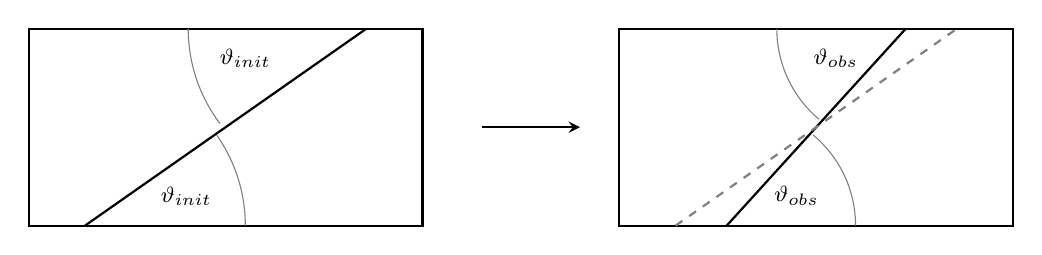
\begin{tikzpicture}[scale=2.5]
			\draw[thick] (0,0) rectangle (2,1);
			\draw[thick] (1-0.5/0.7,0) -- (1+0.5/0.7,1);
			\draw (0.8,0.15) node {\footnotesize$\vartheta_{init}$};
			\draw (1.1,0.85) node {\footnotesize$\vartheta_{init}$};
			\draw[gray] (0.81,1) arc (180:217:0.8);
			\draw[gray] (1.1,0) arc (0:35:0.8);
			
			\draw[thick,-stealth] (2.3,0.5) -- (2.8,0.5);
			
			\draw[thick] (3,0) rectangle (5,1);
			\draw[thick] (4-0.5/1.1,0) -- (4+0.5/1.1,1);
			\draw[dashed,gray,thick] (4-0.5/0.7,0) -- (4+0.5/0.7,1);
			\draw (3.9,0.15) node {\footnotesize$\vartheta_{obs}$};
			\draw (4.1,0.85) node {\footnotesize$\vartheta_{obs}$};
			\draw[gray] (3.8,1) arc (180:230:0.6);
			\draw[gray] (4.2,0) arc (0:50:0.6);
		\end{tikzpicture}
		\caption[Sketch - tilted line validation of the general NBC controlling interface inclination on the domain boundary]{Validation of the general NBC for control of the inclination angle at the boundary - tilted line simulations (isotropic interface energy). The initial angle $\vartheta_{init}$ evolves towards $\vartheta_{obs}$, while $\vartheta$ is imposed by the boundary condition. In the simulations with inclination-dependent interface energy there was $\vartheta_{init}=\vartheta$, see the text for more details.}
		\label{fig_sketch_tilted_plane_validation}
	\end{figure}
	\begin{figure}
		\centering
		\begin{tikzpicture}
			\node[below right, inner sep=0] (L) at (0,0) {
				\includegraphics[width=0.48\textwidth]{validation_iso_specBC_planar.png}};
			\node[below right, inner sep=0] (R) at (L.north east) {
				\includegraphics[width=0.48\textwidth]{validation_aniso_specBC_planar_final.png}};
				
			\draw[above ] (L.north west) node {(a)};
			\draw[above ] (R.north west) node {(b)};
		\end{tikzpicture}
		\caption[Results of tilted plane validation]{Results of tilted plane validation, as sketched in Figure~\ref{fig_sketch_tilted_plane_validation}. In a) the result with isotropic interface, in b) with anisotropic one. }
		\label{fig_tilted_plane_validation_results}
	\end{figure}
	
	\subsection{Particle on a plane (isotropic interface energy)}
	This section shows the validation simulation of a circular segment on a plane using the above model including control of the interface inclination on the domain boundary and subsequent application of the domain scaling method for determination of the shape factor $S$ for this shape. Hence, it is a combined validation of the contact angles reproduction in a more practical simulation than the one with the tilted line, the domain scaling method and also the volume conservation.
	
	In heterogeneous nucleation with isotropic interface energy in 2D, the equilibrium shape is a circular segment and the shape factor as function of the tangent contact angle (wetting angle) $\vartheta$ (see Figure~\ref{fig_sketch_domain_scaling_PF}) is
	\begin{equation}
		S(\vartheta) = \frac{2\vartheta - \sin(2\vartheta)}{2\pi} \,.
	\end{equation}
	A series of phase field simulations was run in the geometry as in Figure~\ref{fig_sketch_domain_scaling_PF} with $\vartheta_L=\vartheta_R$ to assess the above dependence of shape factor on the wetting angle. See Table~\ref{tab_PF_NPA_param_particle_onplane} for details on the simulation grid in the respective simulations. The simulation was terminated when the total interface energy converged. Total interface energy was not evaluated at every time step, but only at evenly distributed logging points. The condition for termination due to convergence in energy was that the relative difference of the current energy value from the mean of the last 10 logging points was less than $5\cdot 10^{-4}$. Two examples of the resulting shapes are provided in Figure~\ref{fig_result_NPA_PF_simulated_shapes}.
	\begin{table}
		\centering
		\caption[PF wetting simulation of a particle with isotropic interface energy - simulation grid dimensions]{Simulation grid dimensions in individual simulations of a particle with isotropic interface energy on a plane in 2D. The grid aspect ratio was determined based on the expected shape aspect ratio.}
		\label{tab_PF_NPA_param_particle_onplane}
		\begin{tabular}{c|c}
			$\vartheta$ & $N_x\times N_y$ \\ \hline
			15	&	$546\times 42$	\\
			30	&	$382\times 51$	\\
			45	&	$308\times 64$	\\
			60	&	$261\times 75$	\\
			75	&	$226\times 87$	\\
			90	&	$198\times 99$	\\
			105	&	$176\times 111$	\\
			120	&	$162\times 121$	\\
			135	&	$152\times 129$	\\
			150	&	$145\times 135$	\\
			165	&	$141\times 139$	
		\end{tabular}
	\end{table}
	
	\begin{figure}
		\centering
		\begin{tikzpicture}
			\draw node (1) at (0,0) {\includegraphics[width=0.49\textwidth]{NPA_PF_phase_field_ang45.pdf}};
			\draw node[below right] (2) at (1.north east) {\includegraphics[width=0.49\textwidth]{NPA_PF_phase_field_ang150.pdf}};
			\draw node[inner sep =0, below right] at (1.north west) {(a)};
			\draw node[inner sep =0, below right] at (2.north west) {(b)};
		\end{tikzpicture}
		\caption[Results - simulated shapes in isotropic particle on a plane]{Examples of resulting shapes obtained by phase field simulation of a particle with isotropic interface energy resting on a plane. In (a) with the contact angle $\vartheta = 45$\textdegree, in (b) with $\vartheta = 150$\textdegree. In both, the phase field contour was denoted by solid red line. It was defined as the zero-value contour of $\eta_{liquid}-\eta_{particle}$.}
		\label{fig_result_NPA_PF_simulated_shapes}
	\end{figure}
	
	The contact angles were the same as in the tilted plane validation, i.e. from $\vartheta=15$\textdegree~to $\vartheta=165$\textdegree~with a 15\textdegree~step. The initial condition corresponded to the target circle segments to reduce the computation time. Using the equation~\eqref{eq_NPA_PF_formula} and taking into account that the non-dimensional area for a circle is $\hat{A}_{circle}=\pi$, the results in Figure~\ref{fig_result_NPA_PF_S_iso} were obtained.
	\begin{figure}
		\centering
		\begin{tikzpicture}
			\draw node (1) at (0,0) {\includegraphics[width=0.49\textwidth]{NPA_PF_relerr_fit_perc_iso.pdf}};
			\draw node[below right] (2) at (1.north east) {\includegraphics[width=0.49\textwidth]{NPA_PF_abserr_iso.pdf}};
			\draw node[below right] (3) at (1.south) {\includegraphics[width=0.49\textwidth]{NPA_PF_S_iso.pdf}};
			\draw node[inner sep =0, below right] at (1.north west) {(a)};
			\draw node[inner sep =0, below right] at (2.north west) {(b)};
			\draw node[inner sep =0, below right] at (3.north west) {(c)};
		\end{tikzpicture}
		\caption[Results - shape factor for isotropic particle determined by domain scaling]{Results of the phase field simulation for determination of shape factor in heterogeneous nucleation with isotropic interface energy. In (a) the relative error of the contact angle obtained by fitting the shape by a circle, in (b) the error in observed contact angles evaluated from two contour end points and in (c) the shape factor as obtained by domain scaling method.}
		\label{fig_result_NPA_PF_S_iso}
	\end{figure}
	
	The contours obtained by phase field simulation were fitted by a circle, which provided the radius $R_{circ}$ and the circle center position $(x_{circ},y_{circ})$. A simple derivation delivers the following formula for determination of the contact angle 
	\begin{equation}
		\vartheta = \mathrm{acos}\left(-\frac{y_{circ}}{R_{circ}}\right) \,,
	\end{equation}
	which provided the observed values of contact angle $\vartheta$. In Figure~\ref{fig_result_NPA_PF_S_iso}a, there are relative differences of the observed contact angles from the imposed ones and it can be seen that the overall shapes are reproduced very well. The contact angle was also determined from the contour endpoints, but this yielded significantly greater discrepancy, as can be seen in Figure~\ref{fig_result_NPA_PF_S_iso}b showing the difference between the observed and imposed angles. 
	
	Different settings of the phase field input parameters were compared to eliminate effect of the method itself on the results. In the base run, the interface width was $l_{IW}=$\qty{1e-9}{\m}, with 7 points through the interface. The compared simulations probed the effect of a) increasing the domain area, while keeping the $l_{IW}$ equal (effectively narrowing the physical interface width relative to the simulation initial condition) and of adding points to the interface (both actions refined the grid below the simulated initial condition) and both might improve phase field simulation accuracy in different regards. That did not happen in terms of the contact angles determined by the two contour endpoints, though.
	
	However, the resulting shapes were always reproduced close to the expectation, which is why the shape factor determination was not affected heavily. This is confirmed also by the obtained values of shape factor plotted in Figure~\ref{fig_result_NPA_PF_S_iso}c, which follow closely the analytic prediction. Apparently, only few points near the domain boundary deviated from the expected circular shape. The different interface parametrization mentioned in the previous paragraphs yielded slight improvement in the shape factor values, but not relevant for the current application.
	
	\subsection{Control over interface inclination with inclination-dependent interface energy}
	The tilted plane validation with interface having inclination-dependent interface energy proved that the implementation is working also in this more complicated case. Nevertheless, for demonstration, in Figure~\ref{fig_demo_aniso_paticle_contangs_controlled} there are shown four particles as they were simulated using the model. All of them have the same anisotropic function, but had different (arbitrary) contact angles imposed on both contact points. It can be seen that the interface inclination is indeed controlled.
	
	\begin{figure}
		\centering
		\includegraphics[width=0.7\textwidth]{demonstr_contang_aniso_corr_THESIS.png}
		\caption[Demonstration of control over interface inclination on the domain boundary with anisotropic particle.]{Demonstration of control over interface inclination on the domain boundary with anisotropic particle. All four particles have the anisotropy function $h(\theta)=1+1.625\cos(4(\theta+15))$ and a kind of arbitrary angles were imposed on both sides of the particle, as indicated above each graph.}
		\label{fig_demo_aniso_paticle_contangs_controlled}
	\end{figure}
		

\section{Domain scaling of a particle on a grain boundary intersecting the surface (isotropic interface energy)}
%Here, the equilibrium stable shape is reached in a dynamic simulation. However, in the classical nucleation theory, it is in fact assumed that it stochastically appears due to local energy fluctuations in the nucleation spot. Among all the possible shapes with equal volume, those with lower total interface energy have higher nucleation probability. 
The present section investigates the theoretical case when the nucleus extends over the grain boundary and thus its wetting condition is unequal on the two sides. Such a situation was sketched in Figure~\ref{fig_sketch_particle_onGB}a. The radius of the particle is given by the particle-liquid interface energy and the bulk driving force (see \eqref{eq_crit_radius_2D}), hence the particle tries to emerge/submerge differently on each side of the grain boundary.

\begin{figure}
	\centering
	\begin{tikzpicture}
		\node[below right, inner sep=0] (L) at (0,0) {
			\includegraphics[width=0.48\textwidth]{circles_on_GB.pdf}};
		\node[below right, inner sep=0] (R) at (L.north east) {
			\includegraphics[width=0.48\textwidth]{sketch_geometry_PF_NPA_on_GB.pdf}};
		
		\draw[above ] (L.north west) node {(a)};
		\draw[above ] (R.north west) node {(b)};
	\end{tikzpicture}
	\caption[Sketch - a particle on a grain boundary]{A particle on a grain boundary. In (a) the impact of different wetting on the two sides of the grain boundary is indicated and in (b) the annotations relevant for explanations in text were added: the specific interface energies $\sigma_S^{L/R}$ belong to the substrate-solution interfaces, the grain boundary energies $\sigma_{GB}^{L/R}$ and lengths $l_{GB}^{L/R}$ to the respective grain boundaries and $l_{GB}$ is the total grain boundary length.}
	\label{fig_sketch_particle_onGB}
\end{figure}

The geometry of the resulting problem is sketched in~Figure~\ref{fig_sketch_particle_onGB}b. When the two sides are wetted differently, it implies different contact angles. The curvature $K$ (reciprocal radius) is in principle equal on both sides of the grain boundary, however due to the obvious shape discontinuity it cannot be constant along the whole shape. The chemical potential $\mu_{surf}$ (the capillary driving force, see~\eqref{eq_chempot_constant}) is
\begin{equation}
	\mu_{surf} = \sigma K 
\end{equation}
and must be constant in order to have the stable shape in equilibrium. But for a constant $\sigma$ that cannot be achieved under these conditions. However, the nuclei in classical nucleation theory do not necessarily have the interface-energy minimizing shape, even though that one is the most likely (because it has the smallest nucleation barrier of all shapes). Hence, even if the shape is not in equilibrium, we assume that it could nucleate. Implications of the shape instability are discussed farther, below the results section. 

It was expected that the resulting shape will be some combination of the equilibrium shapes from both sides (see Figure~\ref{fig_sketch_particle_onGB}). To reduce the simulation time, the initial condition was a kind of artificial compound shape: halves of both equilibrium shapes next to each other, connected by a straight line to avoid dents in the shape. The imposed contact angles on both sides were always approximately present already in the initial condition. Two examples of the initial shapes were plotted in Figure~\ref{fig_IC_particle_onGB}.
 
 \begin{figure}
 	\centering
 	\begin{tikzpicture}
 		\node[below right, inner sep=0] (L) at (0,0) {\includegraphics[width=0.48\textwidth]{NPA_PF_onGB_IC_120x45.pdf}};
 		\node[below right, inner sep=0] (R) at (L.north east) {\includegraphics[width=0.48\textwidth]{NPA_PF_onGB_IC_120x75.pdf}};
 		\draw[below right] (L.north west) node {(a)};
 		\draw[below right] (R.north west) node {(b)};
 	\end{tikzpicture}
 	\caption[Initial condition examples for the simulation of a particle on a grain boundary]{Initial condition examples for the simulation of a particle on a grain boundary. In (a) with the contact angles $\vartheta_L = 120$\textdegree, $\vartheta_R = 45$\textdegree, in (b) with $\vartheta_L = 120$\textdegree, $\vartheta_R = 75$\textdegree}
 	\label{fig_IC_particle_onGB}
 \end{figure}

In the computation of the total grain boundary energy (meaning the energy of the substrate-particle interface), there will be two segments now, one on the left and one on the right side from the grain boundary (see Figure~\ref{fig_sketch_particle_onGB}b). These have lengths $l_{GB}^{L}, l_{GB}^{R}$ and specific grain boundary energies $\sigma_{GB}^L=\sigma_{S}^L-\sigma_P\cos(\vartheta_L)$ and $\sigma_{GB}^R=\sigma_{S}^L-\sigma_P\cos(\vartheta_R)$. The symbols $\sigma_{S}^L,\sigma_{S}^R$ stand for the substrate surface energy on either side of the grain boundary and $\sigma_{P}$ is the particle-liquid interface energy. It turns out, that to express the total interface energy change (upon the insertion of the particle on top of the grain boundary) $\Delta G_\sigma$, it is sufficient to assume only $\sigma_P,\vartheta_L,\vartheta_R$, as can be seen below
\begin{align}
	\Delta G_\sigma &= F(\eta,\nabla\eta) + l_{GB}^{L}(\sigma_{GB}^L-\sigma_{S}^L) + l_{GB}^{R}(\sigma_{GB}^R-\sigma_{S}^R) \\
	&= F(\eta,\nabla\eta) - \sigma_P[l_{GB}^{L}\cos(\vartheta_L) + l_{GB}^{R}\cos(\vartheta_R)] \,.
\end{align}

The symbol $F(\eta,\nabla\eta)$ again stands for the total particle-parent phase interface energy. In the general case, the individual segments $l_{GB}^{L}, l_{GB}^{R}$ will have different length, depending on where the grain boundary is positioned below the particle. 

\begin{figure}
	\centering
	\includegraphics[width=\textwidth]{wulff_on_GB.pdf}
	\caption{Illustration of the three considered positions of grain boundary below the nucleus.}
	\label{fig_GB_below_wulff}
\end{figure}

Because the position of the grain boundary below the particle is chosen here, three scenarios were assumed and illustrated in Figure~\ref{fig_GB_below_wulff}. In each of the scenarios, the grain boundary below the particle is placed in a different spot, hence there will be different total interface energy changes upon the particle insertion $\Delta G_\sigma$, which leads to determination of different shape factors eventually. The three scenarios are below in detail

\begin{enumerate}
	\item $l_L = l_R = l_{GB}/2$, then $\Delta G_\sigma = F(\eta,\nabla\eta)- 0.5\sigma_Pl_{GB}[\cos(\vartheta_L)+\cos(\vartheta_R)]$
	\item $l_L = l_{GB}, l_R = 0$, then $\Delta G_\sigma = F(\eta,\nabla\eta)- \sigma_Pl_{GB}\cos(\vartheta_L)$,
	\item $l_L = 0, l_R = l_{GB}$, then $\Delta G_\sigma = F(\eta,\nabla\eta)- \sigma_Pl_{GB}\cos(\vartheta_R)$ and
\end{enumerate}
In the first case, the substrate grain boundary is just in the middle between the contact points. The second and third ones are limiting cases, when the contact point is infinitesimally just behind the substrate grains grain boundary, hence the full substrate-particle grain boundary lays on the either higher- or lower-energy grain. 


See Table~\ref{tab_ISO_on_GB_angles} for details on the simulation The contact angles $\vartheta_L,\vartheta_R$ were input to the simulation. In the presented results, it was assumed that $\vartheta_L=120$\textdegree and $\vartheta_R$ was varied between 30\textdegree-90\textdegree.

\begin{table}
	\centering
	\caption[PF wetting simulation of a particle with isotropic interface energy ona a GB - contact angles and the simulation grid]{Summary of the contact angles and the simulation grid dimensions in grid points for the simulation of a particle on a grain boundary. Other parameters for the simulation are equal as in Table~\ref{tab_parameters_PF_NPA}.}
	\label{tab_ISO_on_GB_angles}
	\begin{tabular}{c|c|c}
		\hline
		$\vartheta_L$ (\textdegree) & $\vartheta_R$ (\textdegree) & $N_x \times Ny$ \\ \hline
		120 & -30 & $140\times65$ \\
		120 & -45 & $130\times65$ \\
		120 & -60 & $110\times65$ \\
		120 & -75 & $110\times65$ \\
		120 & -90 & $110\times65$ 
	\end{tabular}
\end{table}

\begin{figure}
	\centering
	\includegraphics[width=\textwidth]{comb_ISO_on_GB_contours_evolution.pdf}
	\caption[Time evolution of phase field contours in the simulation of a particle on a grain boundary]{Time evolution of phase field contours in the simulation of a particle on a grain boundary. The time evolves from gray to black contours, the last contour in the simulation is red.}
	\label{fig_PF_nuclbarrier_ISO_onGB_contours}
\end{figure}

The first observation from the simulations is that the shape evolves, but even when it stops evolving, it moves as a block towards the side which has lower grain boundary energy. For the time evolution of the phase field contours in different cases see Figure~\ref{fig_PF_nuclbarrier_ISO_onGB_contours}. The intuitively correct direction of motion (i.e. such which lowers the total grain boundary energy) is reproduced by the model, even though the system energy minimized in the phase field simulation does not account for the particle-substrate interface explicitly. The reason is that the curvature driving force acts towards the center of curvature and as can be seen in Figure~\ref{fig_PF_nuclbarrier_ISO_onGB_contours}, the side with greater contact angle (and thus higher grain boundary energy) is more curved. The flatter is the opposite side, the less is the curvature driving force balanced. 

The velocity of the shape centroid in the x direction was obtained from linear fit through the x centroid coordinate in time, see Figure~\ref{fig_PF_nuclbarrier_ISO_onGB_results}a. The result quantifies the above reasoning, as it can be seen that lower $\vartheta_R$ (i.e. flatter right side) were associated with faster translation to the right.

\begin{figure}
	\centering
	\begin{tikzpicture}
		\draw node[below right,inner sep=0] (l) at (0,0) {\includegraphics[width=0.48\textwidth]{PF_nuclbarr_ISO_onGB_centroidVx.pdf}};
		\draw node[below right,inner sep=0] (r) at (l.north east) {\includegraphics[width=0.48\textwidth]{PF_nuclbarr_ISO_onGB_SFrange.pdf}};
		\draw node[inner sep=0,right] at (l.north west) {(a)};
		\draw node[inner sep=0,right] at (r.north west) {(b)};
	\end{tikzpicture}
	\caption[Results from the simulation of a particle on a grain boundary - velocity of shape motion and the shape factor]{Results from the simulation of a particle on a grain boundary. In (a) the x-direction velocity of the shape centroid as function of the right contact angle $\vartheta_R$ and in (b) the shape factor corresponding to the shape at the end of the simulation (i.e. red contours from Figure~\ref{fig_PF_nuclbarrier_ISO_onGB_contours}) compared to the shape factors for the equilibrium shapes on either the low-energy (solid black line) or high-energy (dashed black line) side of the grain boundary within the substrate. As explained in the text, position of the substrate grain boundary strongly affects the shape factor, hence it is shown as the red area for the phase field simulation results $S_{PF}$. The red line in the center corresponds to the case when the grain boundary was in the middle of the particle.}
	\label{fig_PF_nuclbarrier_ISO_onGB_results}
\end{figure}

The computed shape factors of the compound shapes were plotted in Figure~\ref{fig_PF_nuclbarrier_ISO_onGB_results}b as red area indicating the possible span of values depending on the grain boundary position below the particle. In the same figure, the shape factors corresponding to the shapes nucleating on either side of the substrate grain boundary were indicated by a black dashed line for the high-energy side and a solid black line for the lower-energy side. The grain boundary energy contribution in the total energy of the particle (now understand the grain boundary between the particle and substrate) seems to be a crucial factor for the nucleation probability. When the particle is sufficiently shifted to she lower-energy side, the deviation in shape may not cause dramatic increase in the nucleation barrier. In the opposite case (the particle is rather on the high-energy side), the nucleation can even be less likely than that of an isolated particle (homogeneous nucleation, $S=1$). In the extreme high-energy case for nearly all simulated $\vartheta_R$, the nucleation on top of the boundary was less likely than simply nucleating only on the high-energy part of the substrate. 

An effort was made to characterize the obtained shapes using Bézier polynomials, which are often used in computer graphics and for description of both smooth curves and those with corners. The used method minimized the sum of squared differences between the contour and points on Bézier curve by optimization of the Bézier polynomial control points (the blue circles connected by dashed blue line in Figure~\ref{fig_ISO_on_GB_Bezier_fit}). The used method was linear, hence the handles could be obtained in a single computational step and represent the best match of the chosen order of polynomial to the data.

\begin{figure}
	\centering
	\includegraphics[width=\textwidth]{comb_ISO_on_GB_Bezier_fit.pdf}
	\caption[Fit of the final PF contours of a particle on top of a grain boundary using Bézier polynomials]{Using Bézier polynomials of various orders to fit the contour of a particle on top of a grain boundary. In (a), (c), (e) the contours from simulation with contact angles $\vartheta_L=120$\textdegree and $\vartheta_L=-30$\textdegree fitted using the Bezier polynomial of order $n=3,4,5$, respectively. In (b), (d), (f) the same orders of Bezier polynomials were applied to contours with contact angles $\vartheta_L=120$\textdegree and $\vartheta_L=-90$\textdegree.}
	\label{fig_ISO_on_GB_Bezier_fit}
\end{figure}

\begin{table}
	\centering
	\caption[PF wetting simulation of a particle with isotropic interface energy ona a GB - comparison of measured contact angles]{Comparison of the contact angles in the two simulations which are shown fitted by Bézier polynomials in Figure~\ref{fig_ISO_on_GB_Bezier_fit}. All values are shown in degrees~\textdegree. In column BC the angles are as imposed by the boundary condition, in OBS how they were observed based on the slope between the last two points on the contour on either end, and then based on the control points of the Bézier polynomial od degree $n$.}
	\label{tab_ISO_on_GB_angles_measured}
	\begin{tabular}{c|c|c|c|c|c}
		angle & BC  & OBS & $n=3$ & $n=4$ & $n=5$\\ \hline \hline
		$\vartheta_L$ & 120 & 118.0 & 91.6 & 116.5 & 129.3 \\
		$\vartheta_R$ & -30 & -30.4 & -51.7 & -13.8 & -34   \\ \hline \hline
		$\vartheta_L$ & 120 & 118.0 & 110.7 & 128.1 & 125.7 \\
		$\vartheta_R$ & -90 & -89.4  & -102.0 &-96.8 & -85.0 \\ \hline \hline
	\end{tabular}
\end{table}

The shapes seem rather simple so it was expected that the cubic Bézier polynomial ($n=3$) might suffice for their description, but the match was in fact not very good (see examples in Figure~\ref{fig_ISO_on_GB_Bezier_fit}a and \ref{fig_ISO_on_GB_Bezier_fit}b). Especially the contact points were notably off. The contours were then fitted by Bézier polynomials of orders 4 and 5 to confirm, whether an improvement was possible this way. The polynomials of order 5 provided qualitatively good match to the contours, even though some minor inaccuracy still remained (see Figure~\ref{fig_ISO_on_GB_Bezier_fit}e and \ref{fig_ISO_on_GB_Bezier_fit}f). 

The inaccuracy in Bézier polynomial fit to the contours can be noted on the contact angles the fitted curve had, see Table~\ref{tab_ISO_on_GB_angles_measured}. For all the used orders it can be seen that there is some discrepancy.

Because the Bézier polynomials do not have any physical interpretation in this context, the particular relation of the polynomial control points to the simulation input parameters was not investigated further. However, it can certainly be concluded that the shapes minimizing the isotropic solid-liquid interface energy resting on top of a grain boundary intersecting a planar surface can at least be approximated by Bézier curves of fifth order.

\section{Discussion}
The domain scaling methodology was used to provide the shape factor for the hypothetical case of a particle on top of a grain boundary within otherwise planar surface. As mentioned before, such shape is not the equilibrium one, because for the isotropic particle-solution interface energy $\sigma_P$ it cannot achieve constant curvature, hence in this context a constant chemical potential along the particle surface. 

Given sufficiently large local energy fluctuation, such shapes which do not minimize the interface energy may occur in nucleation. Within the context of classical nucleation theory, the particle is assumed to appear at once. Once it occurs on the grain boundary as presented here, it is unstable and thus should either dissolve, separate into two smaller pieces on either side of the grain boundary (and then probably dissolve due to being of too small to overcome the nucleation barrier) or slide to the lower-energy side of the boundary and attain the energy minimizing shape there. Motion of very mall clusters on a surface during electrodeposition was observed experimentally~\cite{Ustarroz2013}. The sliding scenario is in principle imaginable with liquids but is questionable with continuum-like solids, considered here. 

The splitting scenario is in fact very unlikely in liquids as well, because it would require spontaneous creation of new interface on the particle-liquid interface and simultaneous neglection of the jump in interface energy between the particle and substrate. The jump in interface energy will drive the system to expand the low-energy area on the expense of the high-energy area. In fact, the above simulations results showed that the interface energy acting on the compound equilibrium (unstable) shapes was moving them, not splitting. All the particle interfaces are thus subject to forces acting in the direction to the lower energy substrate side. This means that the particle is either expected to dissolve or to slide towards the low-energy side of the grain boundary on the substrate surface.

The taken approach is in fact not convenient for description of a solid phase nucleation on top of a grain boundary. Even though the exact mechanisms of the nucleation in grain boundaries during deposition are not known, it is more meaningful to imagine such growth rather on the atomic level than assuming the continuum-like nuclei. What is more, the grain boundary width in reality may be of comparable size like the nucleus. That implies that i) the assumption of infinitesimally narrow jump in surface properties is too simplistic and ii) that the grain boundary itself must interact with the particle in some way. Possibly by enabling nucleation in place of some local defect in the grain boundary. Additionally, given the assumed continuum aspect of the particle and its solid state, the only viable resolution of the shape instability in 2D is to dissolve straight away.

In 3D, the grain boundary intersecting the substrate surface can be seen as a triple junction, a line defect which has its energy as well~\cite{Milchev2002}. Upon insertion of the nucleus, part of this line energy would be replaced by the line energy of the triple junction between the two grains and the nucleated particle. If the triple junction with the environment had higher energy than the triple junction with the particle, a reduction in the triple junction line energy would occur in the system. However, it is out of the scope of this work to hypothesize to what extent this might become a factor in (meta)stabilization of the particle. 

However, should the nucleating phase be liquid (e.g. electrodeposited eutectic gallium-indium alloy~\cite{Monnens2023}, the present study has shown that nucleation of the shape which mostly rests on the low-energy side of the substrate surface (while still being in contact with the high-energy side) is comparably probable like nucleation on the low-energy side alone. This can be seen on proximity of the lower edge of the red area in Figure~\ref{fig_PF_nuclbarrier_ISO_onGB_results}b to the solid black line indicating the shape factor the shape nucleating straight on the low-energy side of the substrate. 

\section{Limitations of the presented methodology}
One of the methodology limitations is that sharp angles of the interface inclination require finer grids, because the interface width is finite in the phase field simulation and its projection to the domain boundary can be long with the sharp angles. In fact, the sharpest simulated contact angle in this study was 15\textdegree. That may suffice in many applications with isotropic interface energy, but should a Wulff shape be simulated in arbitrary configuration, even sharper angle might be needed depending on the particle orientation. Using a finer grid should solve the related problems, but the validations have not been carried out and the method already is rather computationally intensive, especially when compared to the Winterbottom construction.

One of the reasons to use the multi-phase field model is that in principle multiple grains or particles could be simulated. However, the interface-inclination-controlling boundary condition assumes that no triple junction is near the interface-boundary contact point. Therefore, until this is somehow resolved, the advantage of using multi-phase field model for this purpose is limited. 

A remark is due towards the original intended application of the methodology, i.e. to bring insight into the nucleation barrier anisotropy. As presented in the next chapter, the basis for that is an analytic model relating the local interface energetics to the local crystallographic orientations of the particle and the substrate. Then it is possible to say how the shape wets the surface and what are the contact angles, hence the equilibrium shape could be obtained using this methodology. However, the insight may only be obtained by probing the substrate and particle orientation space, which implies large number of simulations at similar, yet unequal conditions. The domain scaling methodology would in principle be usable for the purpose, but at some points it would probably hit its limits, because it may not be so accurate in delivering minute details and it is not clear how well it would handle the cases with the contact points close to each other and other scenarios. Additionally, for a single pair of substrate-particle orientations there may be multiple stable solutions, each of which would have to be simulated in order to select the most likely one. 

%It is reasoned, that the Key objective KO2 is met ("\textit{Develop a methodology based on the multi-phase-field model~\cite{Moelans2008} capable of determining the nucleation barrier anisotropy}"), because the phase field model was validated and demonstrated control over the inclination angles also when the interface had the inclination-dependent interface energy. Also, it was demonstrated that no assumption on the resulting shape is needed for determination of the shape factor. Hence, the phase field model in conjunction with the domain scaling method is capable of determining the shape factors for the anisotropic particles which was the objective.

\section{Conclusion}
In this chapter, the author developed and implemented a novel method for determination of a shape factor of a heterogeneous nucleus seen within the framework of classical nucleation theory. This domain scaling method takes as input the contour of the shape on a plane. In combination with the phase-field model which implicitly tracks the interface it is possible to determine shapes of particles on a plane, where the equilibrium stable shape is not a-priori known e.g. from the Winterbottom construction. The case of a particle with isotropic interface energy on a grain boundary where the analytical solution was not known was analyzed. 

In order to deliver the contours to the domain scaling method, the existing multi-phase field model~\cite{Moelans2008, Minar2022} was extended in several regards to allow such simulation. Importantly, volume conservation and general Neumann boundary conditions for control of interface inclination on the domain boundary were added. The model was systematically validated in several benchmarks.

The main results of the investigation of the particle with isotropic interface energy on top of the grain boundary within the substrate are the following:
\begin{itemize}
	\item Shape factors were obtained for five different cases of particles on top of grain boundary,
	\item Position of the substrate grain boundary below the particle strongly determined the shape factor, hence the nucleation probability,
	\item When most of the particle rests on the low-energy side, the shape factor was comparable to the heterogeneous nucleation on the lower-energy side,
	\item The shapes which minimized the particle-liquid interface energy could be well approximated by Bézier polynomials of 5th order, but no physical interpretation was provided. The match could be probably improved by further increasing the order of the polynomial, but no added value was seen in that,
	\item The simulated contours moved towards the lower-energy side of the simulated domain, but it was explained that it was only due to the shape of the contour together with the curvature driving force, not because the simulation would explicitly include the particle-substrate energetics (only the contact angles are the input to the simulation).
\end{itemize}

%%%%%%%%%%%%%%%%%%%%%%%%%%%%%%%%%%%%%%%%%%%%%%%%%%
% Keep the following \cleardoublepage at the end of this file, 
% otherwise \includeonly includes empty pages.
\cleardoublepage

% vim: tw=70 nocindent expandtab foldmethod=marker foldmarker={{{}{,}{}}}
